\section{Resource Access Protocol}

Now we will discus 2 main resource access protocol for periodic task which are:

\begin{itemize}
\item Non-Preemptive Protocol
\item Highest Locker Priority

\end{itemize}


The first protocol is for non-preemptive-able scheduler and the second protocol is for preemptive-able scheduler. The following list are the important notation that I will use in explaining each protocol. The main idea about those protocol is to avoid priority invention, so that the blocking time experienced by the task that have highest priority by lower priority task will also be discussed for each protocol.

\begin{itemize}
\item $ B_{i} $ denotes the maximum blocking time task $ \tau_{i} $ can experience.
\item $ z_{i,k} $ denotes a generic critical section of task $ \tau_{i} $ guarded by semaphore $ S_{k} $.
\item  $ Z_{i,k} $ denotes the longest critical section of task $ \tau_{i} $ guarded by semaphore $ S_{k} $.
\item $ \delta_{i,k} $ denotes the duration of $ Z_{i,k} $.
\item $ z_{i,h} \subset z_{i,k} $ indicates that $ z_{i,h} $ is entirely contained in $ z_{i,k} $.


%\item $ \sigma_{i} $ denotes the set of semaphores used by $ \tau_{i} $.
%\item $ \sigma_{i,j} $ denotes the set of semaphores that can block $ \tau_{i} $, used by the lower-priority task $ \tau_{j} $ .
%\item $ \gamma_{i,j} $ denotes the set of the longest critical sections that can block $ \tau_{i} $, accessed by the lower %priority task $ \tau_{j} $ . That is,
%\begin{center}
%$ \gamma_{i}=\{Z_{j,k} | P_{j}<P_{i}$ and $(S_{k}\geq \sigma_{i,j}) \} $
%\end{center}
%\item $ \gamma_{i}$ denotes the set of all the longest critical sections that can block $ \tau_{i} $. That is,
%\begin{center}
%$ \sigma_{i} =\underset{j:P_{j}>P_{i}}{\cup} \gamma_{i,j}$
%\end{center}

\end{itemize}


\section{Non-Preemptive Protocol}

In this section, I will explain about Non-Preemptive Protocol.

\subsection{Definition}

This protocol is a simple protocol and named non-preemptive(NP) because it avoids any interruption on running task $\tau_{j}$ that accessing a resource $ R_{k} $that guarded by , $ S_{k} $. To reduce total blocking time experienced by the task $\tau_{i}$ that have the highest priority, this protocol just increase the priority of the task $\tau_{j}$ that currently accessing the resource $ R_{k} $, so that the task will not be interrupted and can be done much faster.Without this protocol, the task that highest priority $\tau_{i}$ will interrupt the task $\tau_{j}$ that currently accessing the resource $ R_{k} $ even though the task cannot access the resource because it already guarded by $ S_{k} $. The scheduler then switch back to the task before to finish its process, this switch context process could cause longer blocking time experienced by the highest priority task. After the task$\tau_{j}$ finish accessing the resources, its priority will be back to its nominal priority $ P_{j} $.These situations can be compared through ``Fig. \ref{fig:An_example_of_priority_inversion}'' and ``Fig. \ref{fig:Example_of_NPP_preventing_priority_inversion}''. So, the priority of the task $\tau_{j}$that currently accessing the resource is 

\begin{equation}
\citeequation{p_{j}(R_{k})=\underset{h}{\mathrm{max}}\{P_{h}\}}{b5}\label{eq5}
\end{equation}

\begin{figure}[ht]
    \centering
    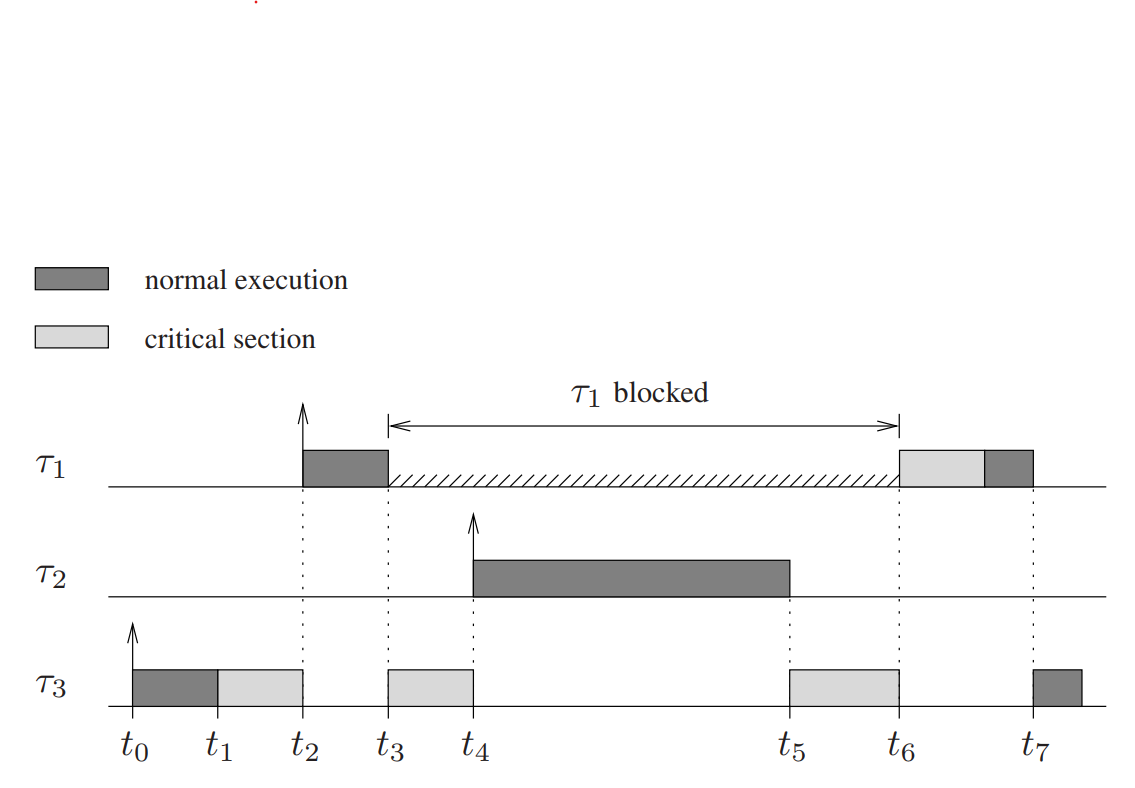
\includegraphics[width=0.5\textwidth]{An_example_of_priority_inversion}
    \caption{An example of priority inversion.. \cite{b5}}
    \label{fig:An_example_of_priority_inversion}
\end{figure}

\begin{figure}[ht]
    \centering
    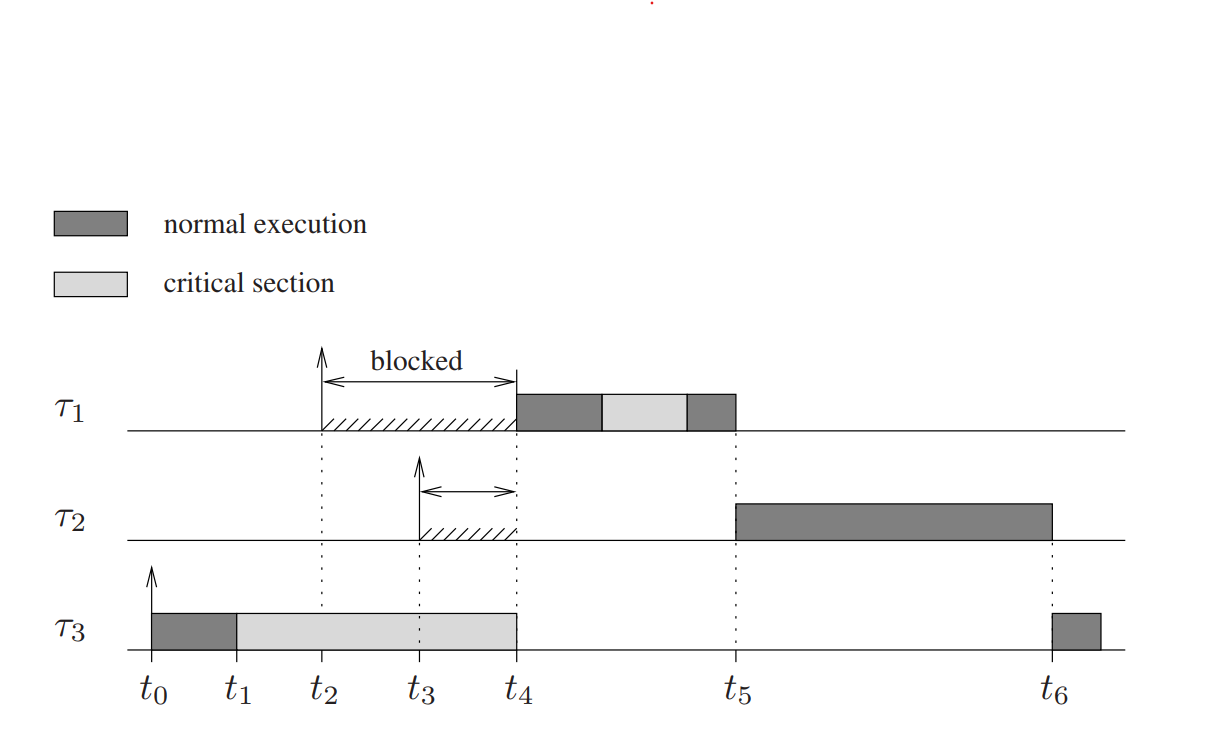
\includegraphics[width=0.5\textwidth]{Example_of_NPP_preventing_priority_inversion}
    \caption{Example of NPP preventing priority inversion. \cite{b5}}
    \label{fig:Example_of_NPP_preventing_priority_inversion}
\end{figure}


\subsection{Blocking time computation}

	The total of critical section of lower priority task $\tau_{j}$ blocking higher priority task $\tau_{i}$ is

\begin{equation}
\citeequation{ \gamma_{i}=\{Z_{j,k} | P_{j}<P_{i}, k=1,...,m \}}{b5}\label{eq6}
\end{equation}

From my understanding, the value of k could be more than one if the task that have the highest priority want to access more than one resource and each resource are currently accessed by the task that have lower priority. Hence, in the total duration, the highest priority task is blocked is

\begin{equation}
\citeequation{B_{i}(R_{k})=\underset{j,k}{\mathrm{max}} \{ \delta_{j,k}-1 | Z_{j,k} \in \gamma_{i}\}}{b5}\label{eq7}
\end{equation}


The value of $\delta_{j,k}$is reduced one unit time because the task that have lower priority, $\tau_{j}$ could block the task with the highest priority, $\tau_{i}$ from accessing a resource only and only if the task $\tau_{j}$  arrived at least one unit time earlier than $\tau_{i}$.

\subsection{Implementation Strategies}

As state by \cite{b6} - "All commercial RTOSs have a means for beginning and ending a critical section. Invoking this Scheduler operation prevents all task switching from occurring during the critical section. If we write our own RTOS, the most common way to do this is to set the Disable Interrupts bit on our processor's flags register. The precise details of this vary, naturally, depending on the specific processor."

Means that, this resource access protocol is nothing more than avoiding interrupt on running task. 

Base on the model that I made using UPPALL, it is true that the result in terms of the longest blocking time experienced by the highest priority task in both case, disabling interrupt without NPP and enabling interrupt with NPP is the same. Using the same model, I found that it is possible that a higher priority task could miss deadline without applying NNP while interrupt is enabled. The model can be downloaded from \url{https://github.com/Adib6637/UPPAAL} to see the simulation.

\subsection{Sample Model}

In this section, I will explain the sample model of NPP that I made. For this sample model, I use a clock that can display time and date. Considering the task of displaying date,$\tau_{d}$ have higher priority than task displaying time,$\tau_{t}$ and they share the same resource which is Display unit,$R_{d}$, the scheduler will preempt the task $\tau_{t}$ whenever the task $\tau_{d}$ is ready as shown in ``Fig. \ref{fig:sample_model_without_npp}''.
\begin{figure}[ht]
    \centering
    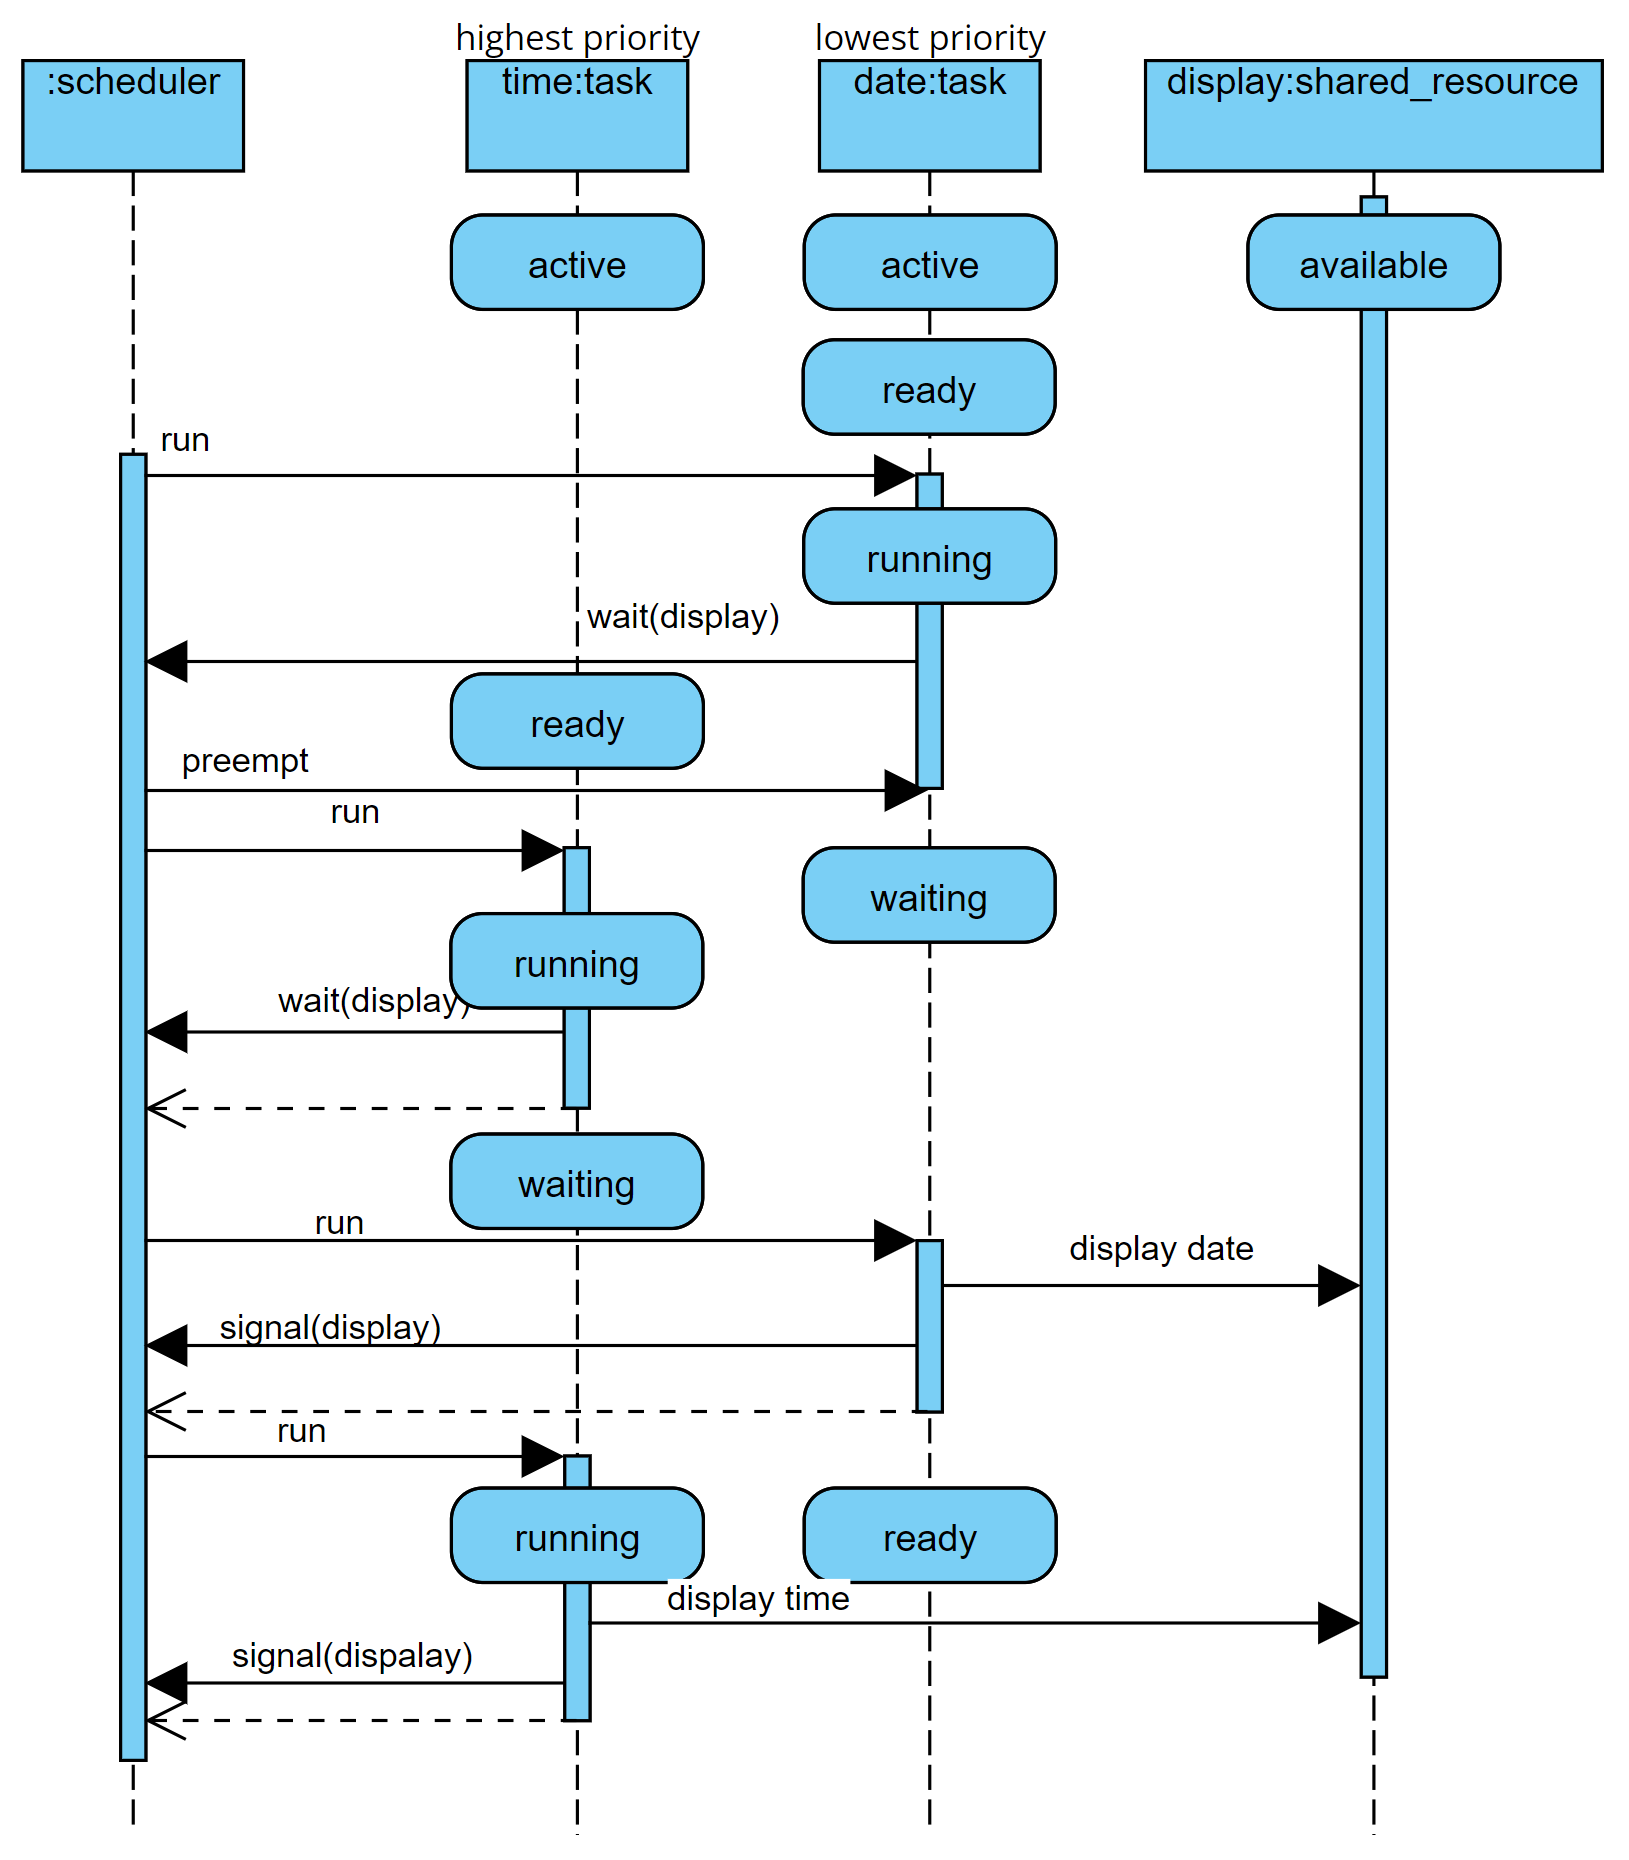
\includegraphics[width=0.5\textwidth]{sample_model_without_npp}
    \caption{Sample Model without Non-Preemptive Protocol} \cite{b6}
    \label{fig:sample_model_without_npp}
\end{figure}

By applying NNP as shown in ``Fig. \ref{fig:sample_model_with_npp}'', the task $\tau_{d}$ cannot be preempted in event the task $\tau_{t}$ is ready because the dynamic priority of the task $\tau_{d}$ is arisen to the highest and back to its nominal value when the task $\tau_{d}$ leave its critical section. 


\begin{figure}[ht]
    \centering
    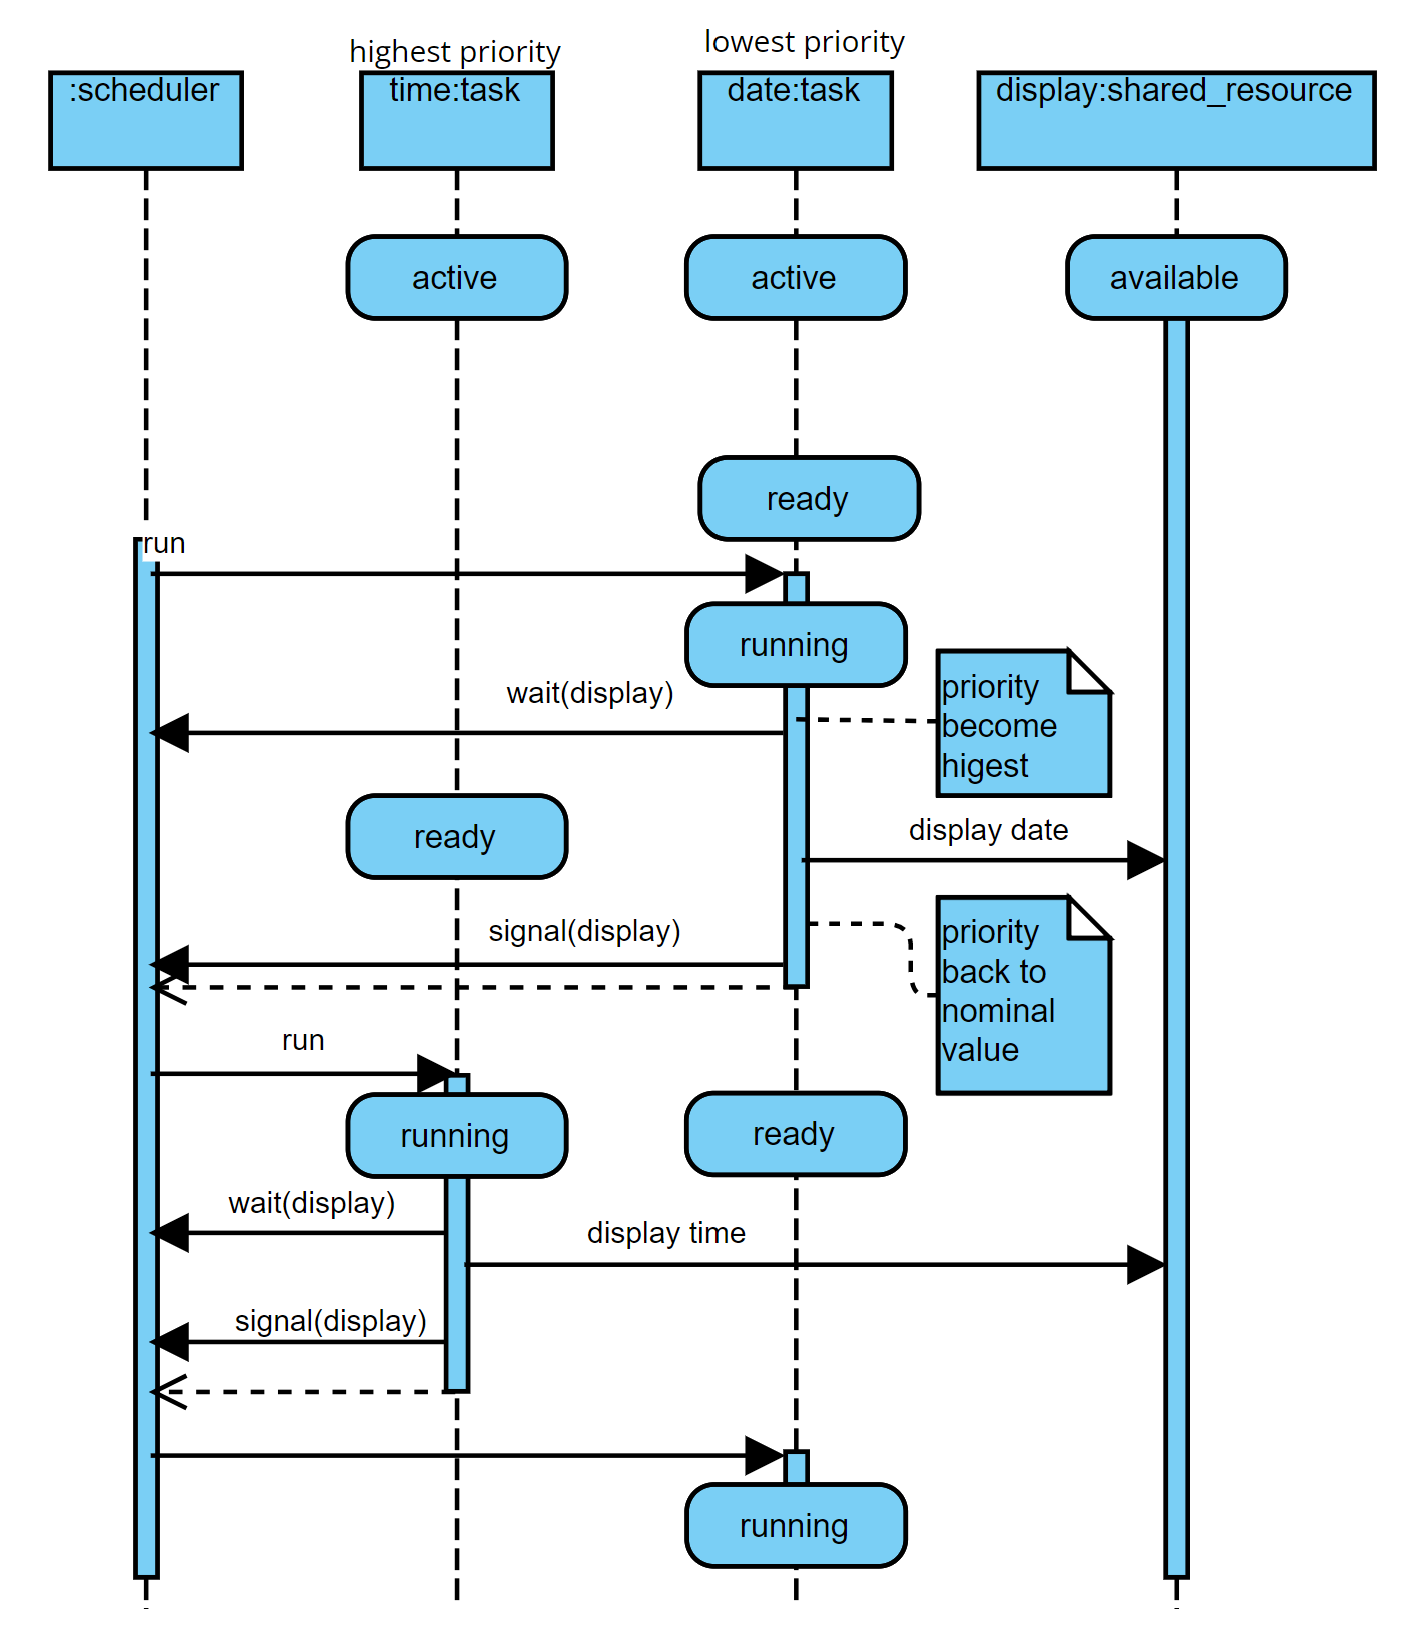
\includegraphics[width=0.5\textwidth]{sample_model_with_npp.png}
    \caption{Sample Model with Non-Preemptive Protocol }
    \label{fig:sample_model_with_npp}
\end{figure}


\subsection{Problem Arise}

As shown in ``Fig. \ref{fig:Example_in_which_NPP_causes_unnecessary_blocking_on_T1}'', this protocol will block the highest priority task $ \tau_{1} $ even though the task will not access the resource because the priority of the task $\tau_{3}$ have been increase to the maximum.

\begin{figure}[ht]
    \centering
    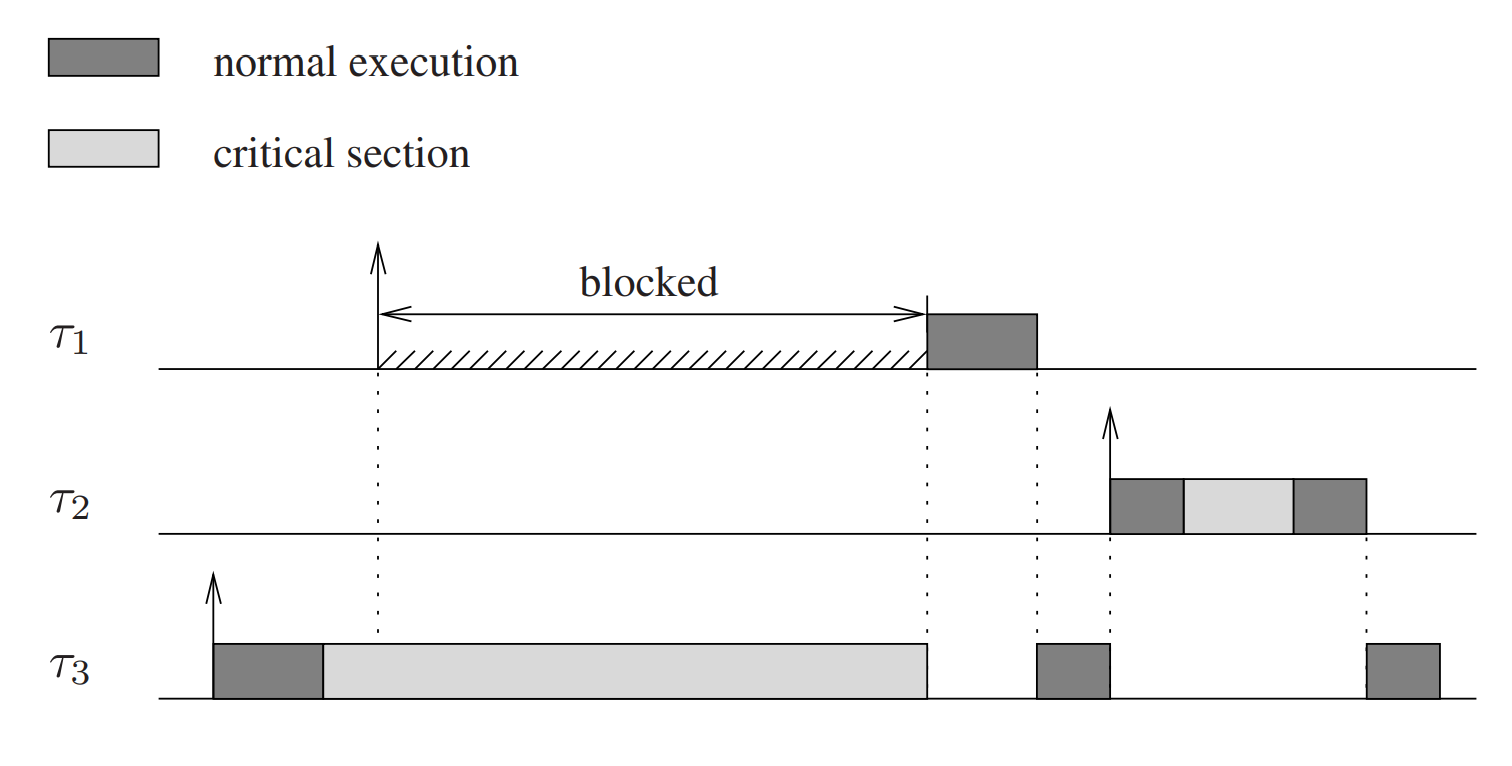
\includegraphics[width=0.5\textwidth]{Example_in_which_NPP_causes_unnecessary_blocking_on_T1}
    \caption{Example in which NPP causes unnecessary blocking on $ \tau_{1} $ \cite{b5}}
    \label{fig:Example_in_which_NPP_causes_unnecessary_blocking_on_T1}
\end{figure}

Back to our sample model, this situation can be illustrated by adding a new task that didn't use the resource,$ R_{d}$ like alarm task, $\tau_{a}$ as shown in ``Fig. \ref{fig:sample_model_problem_npp}''.

 
\begin{figure}[ht]
    \centering
    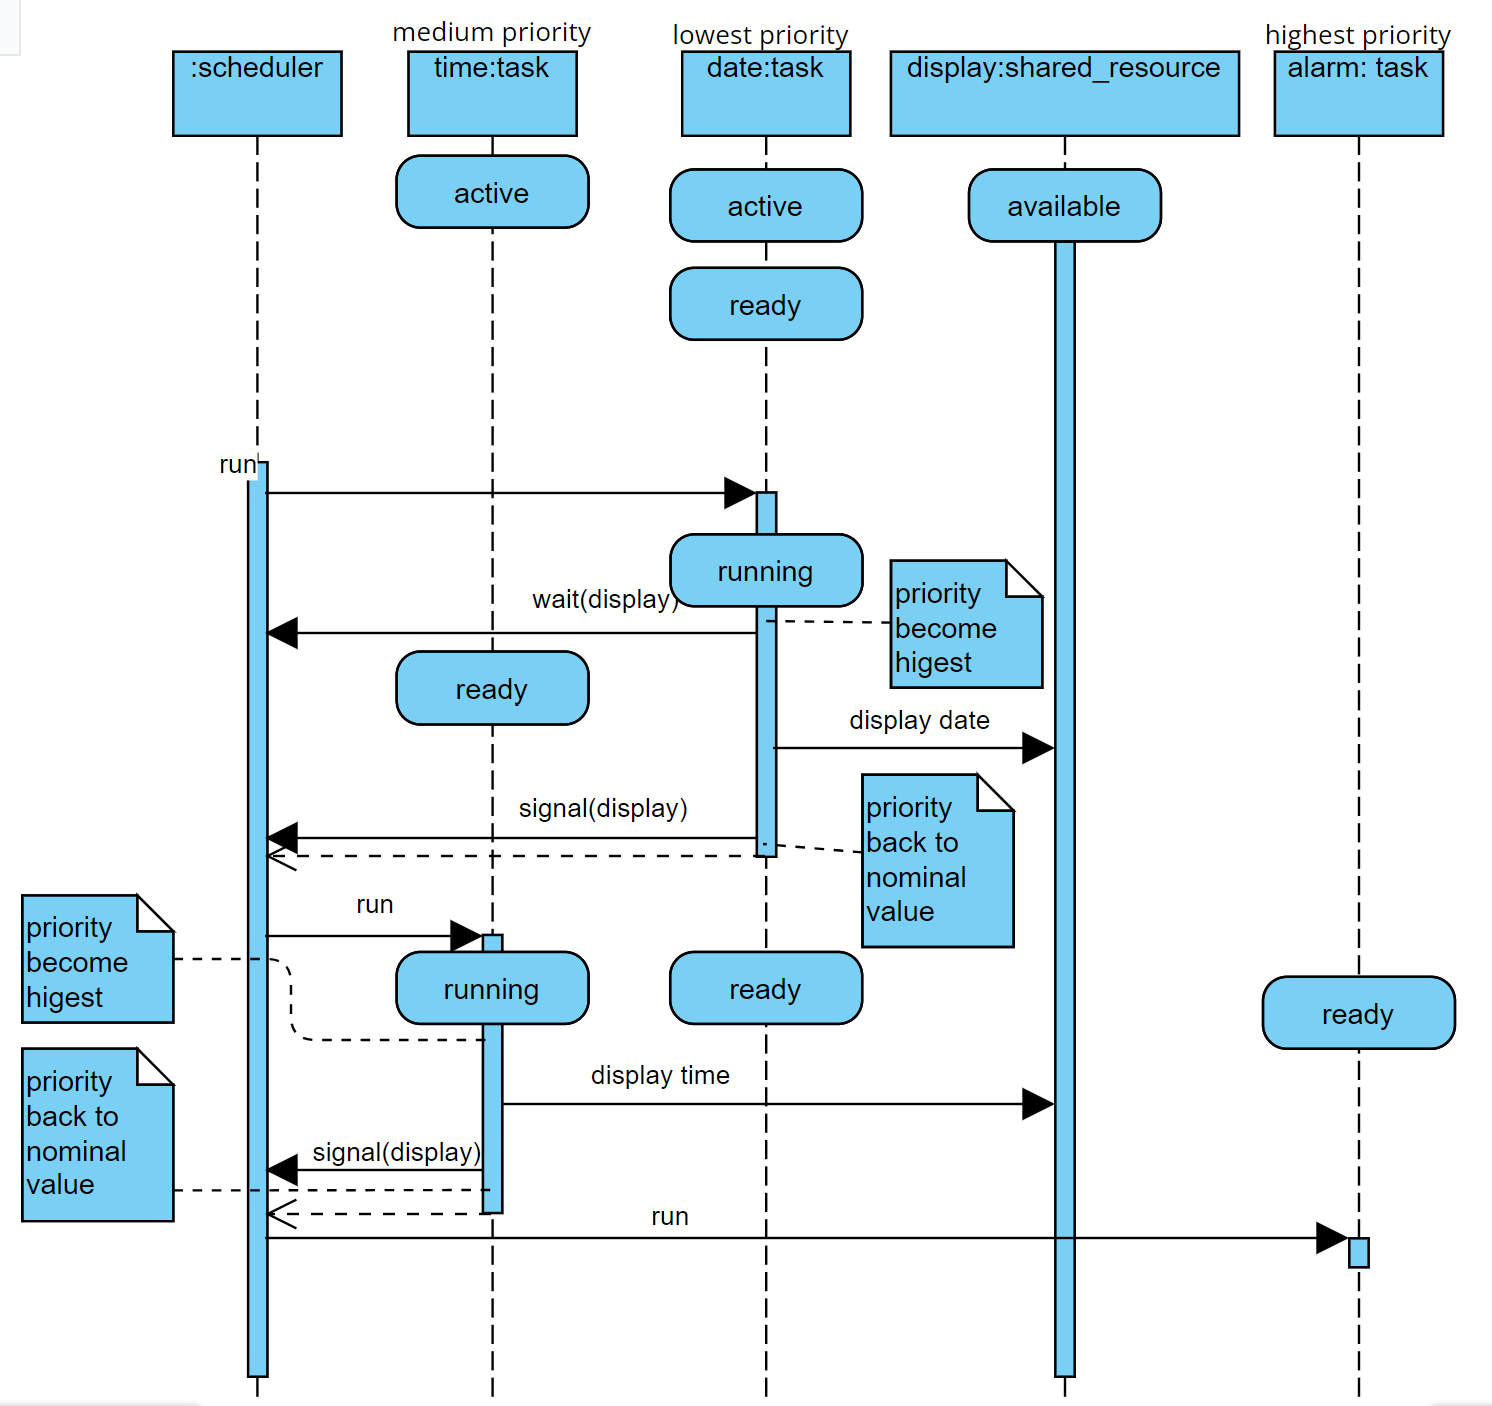
\includegraphics[width=0.5\textwidth]{sample_model_problem_npp}
    \caption{Example in which NPP causes unnecessary blocking on alarm task, $ \tau_{a} $ }.
    \label{fig:sample_model_problem_npp}
\end{figure}

 This problem could be solved by the protocol in the next section, which is Highest Locker Priority (HLP) protocol.
\section{Highest Locker Priority}

\subsection{Definition}

Highest Locker Priority (HLP) is the improvement of the previous protocol to allow the highest priority task $\tau_{i}$ that doesn't use resource $R_{k}$ to interrupt the lower priority task $\tau_{j}$ that use the resource, $R_{k}$ by limiting the raised priority of the task $\tau_{j}$. So, 
 
\begin{center}
 $p_{j}(R_{k})=\underset{h}{\mathrm{max}} \{P_{h}| \tau_{h}$ uses $R_{k}\}  $ \cite{b5}
\end{center}

whereas the priority of task, $\tau_{j}$ that are currently accessing the resource, $R_{k}$ in increased to the maximum only among the task. This dynamic priority then set back to its nominal value $P_{j}$ when the task leave its critical section. The maximum raised priority of a task $\tau_{j}$ is called priority ceiling $ C(R_{k}) $ and computed off-line.  The maximum priority $ C(R_{k}) $ of the tasks sharing $ R_{k} $ is the computed online such

\begin{center}
$C(R_{k})\stackrel{def}{=}\underset{h}{\mathrm{max}} \{P_{h}| \tau_{h}$ uses $R_{k}\}  $ \cite{b5}
\end{center}

Since the priority of lower priority task $\tau_{j}$ is raised as soon as the task entering $ R_{k} $, this protocol also known as Immediate Priority Ceiling. This protocol can be visualized as in figure \ref{fig:Example_of_schedule_under_HLP} where task $ \tau_{1} $ have highest priority and task $ \tau_{3} $ is the first task arrived.

\begin{figure}[h]
    \centering
    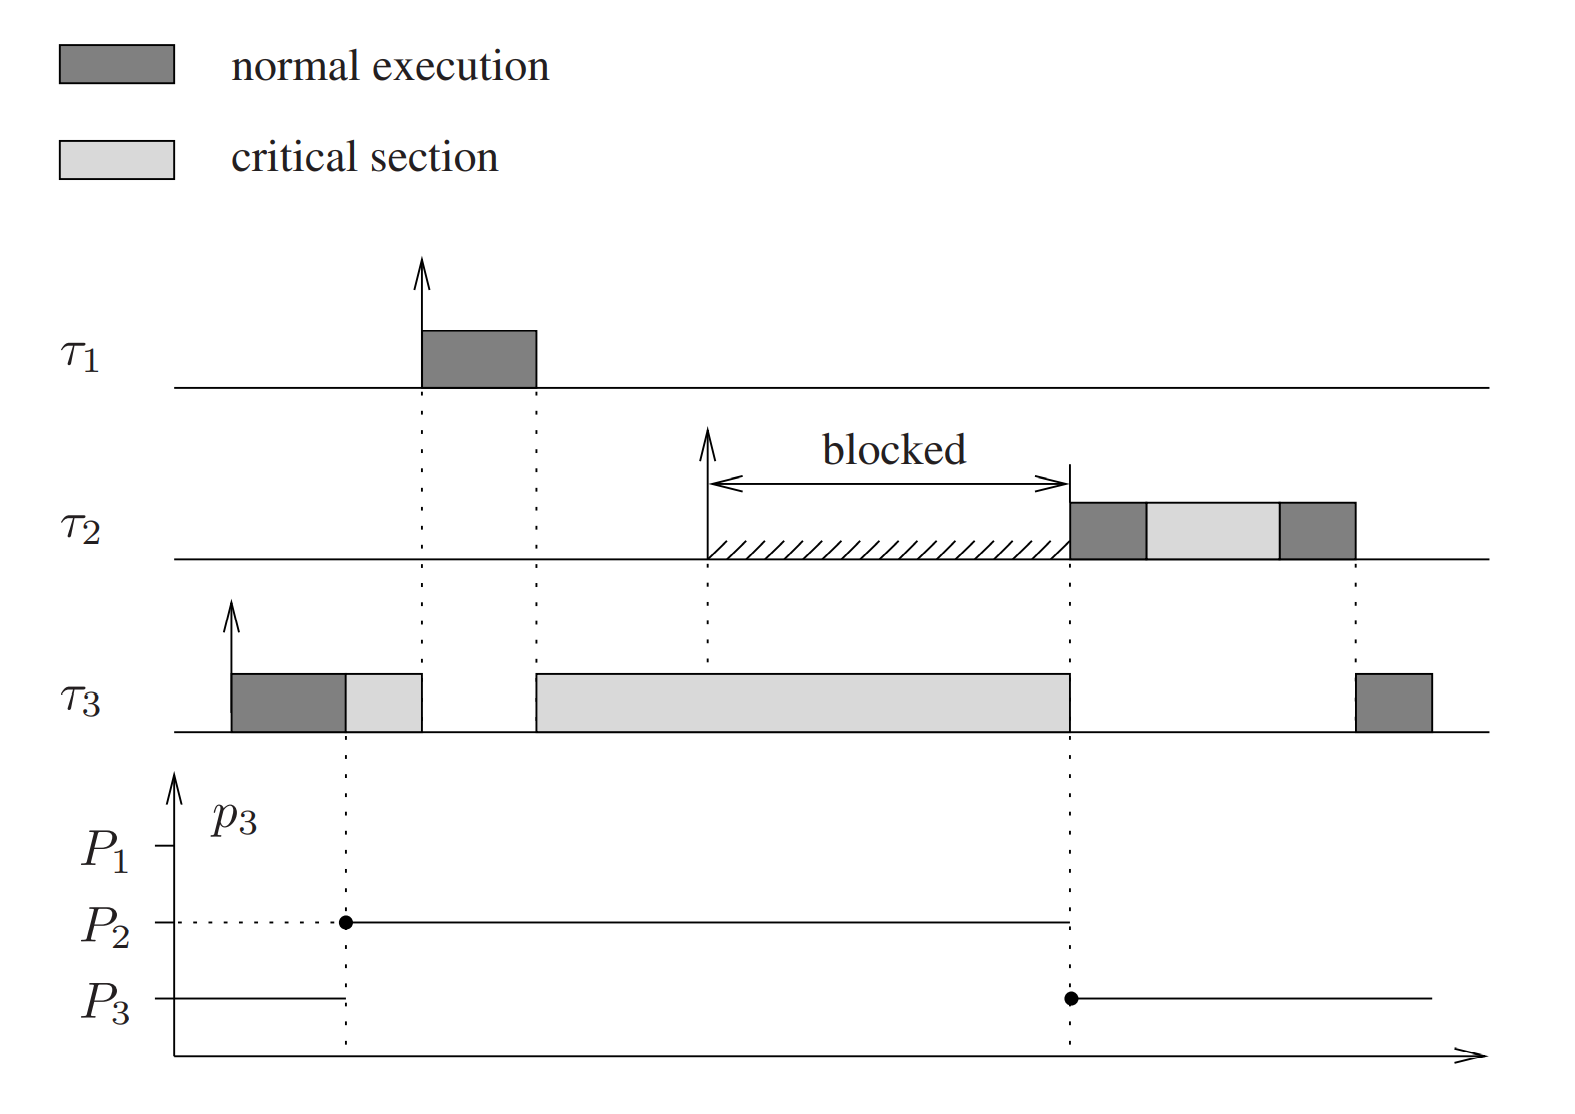
\includegraphics[width=0.5\textwidth]{Example_of_schedule_under_HLP}
    \caption{ Example of schedule under HLP, where $ p3 $ is raised at the level $ C(R) = P_{2} $ as soon as $ \tau_{3} $ starts using resource R \cite{b5}}
    \label{fig:Example_of_schedule_under_HLP}
\end{figure}

 
\subsection{Blocking Time Computation}

The total of critical section of lower priority task $\tau_{j}$ blocking a higher priority task $\tau_{i}$ is reduced by adding a new parameter as shown below. Means that the highest priority task that didn't want to use the resource could not be blocked by the lower priority task that are currently using the resource.

\begin{center}
$ \gamma_{i}=\{Z_{j,k} | P_{j}<P_{i} $ and $ C(R_{k})\geq P_{i} \} $ \cite{b5}
\end{center}

According to \cite{b5} - "Under HLP, a task $ \tau_{i} $ can be blocked, at most, for the duration of a single critical section belonging to the set $ \gamma_{i} $ and this theorem is proved by contradiction".  

As shown in figure \ref{fig:Example_of_schedule_under_HLP}, $ \tau_{i} $ can be blocked at maximum once, means that

\begin{center}
$B_{i}(R_{k})=\underset{j,k}{\mathrm{max}} \{ \delta_{j,k}-1 | Z_{j,k} \in \gamma_{i}\}  $ \cite{b5}
\end{center}

We need to minus one unit of time because the lower priority task $ \tau_{j} $ need to access $ R_{k} $ atleast one unit of time earlier than $ \tau_{i} $ to block it.

\subsection{Implementation Strategies} 

According to \cite{b6} - "Fewer RTOSs support the Highest Locker Pattern more than the basic Priority Inheritance Pattern. The implementation of this pattern  is fairly straightforward, with the addition of priority ceiling attributes in the Shared Resource. When the mutex is locked, it must notify the Scheduler to elevate the priority of the locking task to that resource's priority ceiling."

\subsection{Sample Model} 

In this section, I will explain the sample model of HLP that I made. Our aim now is to solve the problem in Figure\ref{fig:sample_model_problem_npp} by applying HLP. As the result, the dynamic priority of task that currently accessing the resource, $ R_{d}$, which is the display is risen to the highest only among the task that want to access the resource, $ R_{d}$. This solution is illustrated in Figure \ref{fig:sample_model_with_hlp}. So, the task $ \tau_{t}$ can be preempted by the highest priority task, the alarm task, $\tau_{a}$ even though the task is currently accessing the resource $ R_{d}$.


\begin{figure}[h]
    \centering
    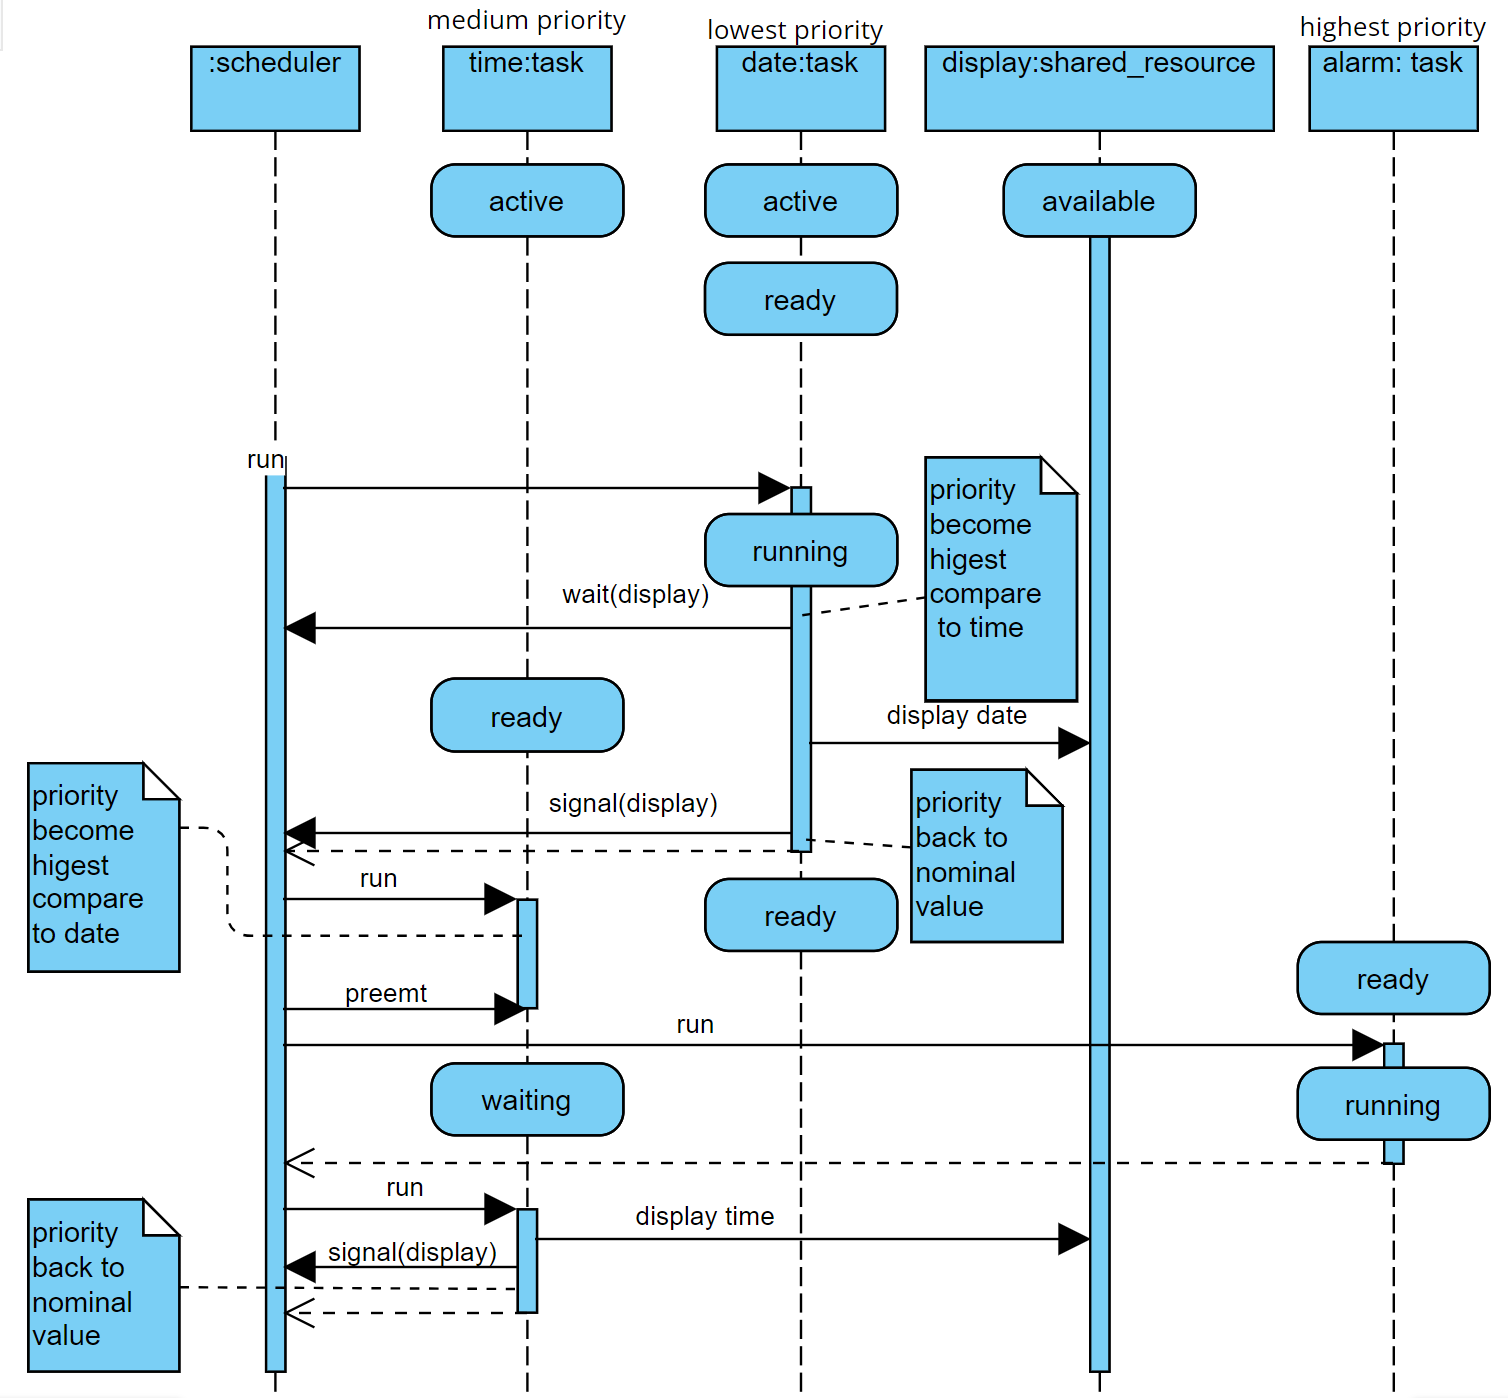
\includegraphics[width=0.5\textwidth]{sample_model_with_hlp}
    \caption{}
    \label{fig:sample_model_with_hlp}
\end{figure}


\subsection{Problem Arise}

As claimed by \cite{b5} -"despite the fact that this algorithm improves the previous algorithm, it still could produce some unnecessary blocking. This algorithm block a task at the time it attempts, before it actually require a resource \cite{b5}. If a critical section is contained only in one branch of a conditional statement, then the task could be unnecessarily blocked, since during execution it could take the branch without the resource."
 










